%!TEX root = ../../main.tex

\chapter{Sequences}
\label{cha:sequences}

A sequence is a list of pictograms, where it is possible to mark a progress in the sequence of pictograms. This components is very common in the Sekvens app and the Ugeplan app.

\section{Progress}
\label{sec:progress}

The progress of the sequence is indicated by the size of pictograms in the sequence. The pictogram currently in progress is marked by upscaling the pictogram a bit like seen in FIGREF.

\todo[inline]{Insert an example of the sequence progress}

\todo[inline]{Describe that sequences (and ``sequences'' used in week schedules) should be as seen in the figure below. Notice that when selecting a specific point in the schedule that this should be centered in the middle. However you should still be able to scroll through the list}

\begin{figure}[!htbp]
		\centering
		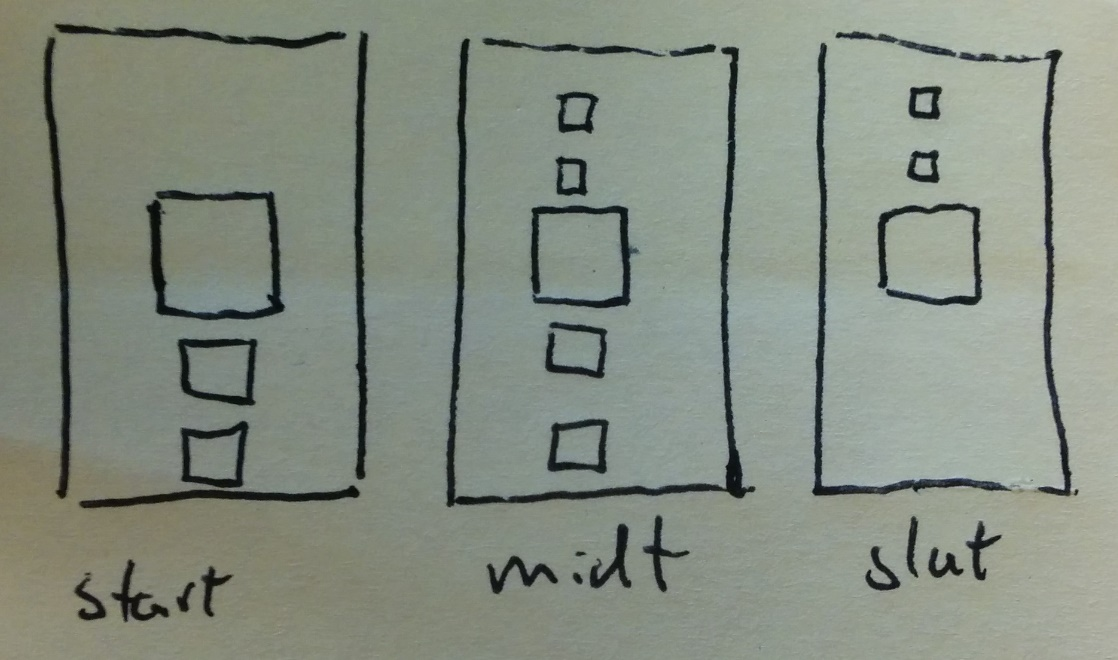
\includegraphics[width=\textwidth]{todo_sequence}
	\end{figure}